 \documentclass[12pt]{exam}

% essential packages
\usepackage{fullpage} % margin formatting
\usepackage{enumitem} % configure enumerate and itemize
\usepackage{amsmath, amsfonts, amssymb, mathtools} % math symbols
\usepackage{xcolor, colortbl} % colors, including in tables
\usepackage{makecell} % thicker \Xhline in table
\usepackage{graphicx} % images, resizing

% sometimes needed packages
\usepackage{hyperref} % hyperlinks
% \hypersetup{colorlinks=true, urlcolor=blue}
% \usepackage{logicproof} % natural deduction
\usepackage{tikz} % drawing graphs
\usetikzlibrary{positioning}
% \usepackage{multicol}
% \usepackage{algpseudocode} % pseudocode

% paragraph formatting
\setlength{\parskip}{6pt}
\setlength{\parindent}{0cm}

% newline after Solution:
\renewcommand{\solutiontitle} {\noindent\textbf{Solution:}\par\noindent}

% less space before itemize/enumerate
\setlist{topsep=0pt}

% creates \filcl to grey out cells for groupwork grading
\newcommand{\filcl}{\cellcolor{gray!25}}

% creates \probnum to get the problem number
\newcounter{probnumcount}
\setcounter{probnumcount}{1}
\newcommand{\probnum}{\arabic{probnumcount}. \addtocounter{probnumcount}{1}}

% use roman numerals by default
\setlist[enumerate]{label={(\roman*)}}

% creates custom list environments for grading guidelines, question parts
\newlist{guidelines}{itemize}{1}
\setlist[guidelines]{label={}, left=0pt .. \parindent, nosep}
\newlist{gwguidelines}{enumerate}{1}
\setlist[gwguidelines]{label={(\roman*)}, nosep}
\newlist{qparts}{enumerate}{2}
\setlist[qparts]{label={(\alph*)}}
\newlist{qsubparts}{enumerate}{2}
\setlist[qsubparts]{label={(\roman*)}}
\newlist{stmts}{enumerate}{1}
\setlist[stmts]{label={(\roman*)}, nosep}
\newlist{pflist}{itemize}{4}
\setlist[pflist]{label={$\bullet$}, nosep}
\newlist{enumpflist}{enumerate}{4}
\setlist[enumpflist]{label={(\arabic*)}, nosep}

\printanswers

\newcommand{\prevhwnum}{7}
\newcommand{\hwnum}{8}

\begin{document}
%%%%%%%%%%%%%%% TITLE PAGE %%%%%%%%%%%%%%%
\title{EECS 203: Discrete Mathematics\\
  Winter 2024\\
  Homework \hwnum{}}
\date{}
\author{}
\maketitle
\vspace{-50pt}
\begin{center}
  \huge Due \textbf{Thursday, April 4}, 10:00 pm\\
\Large No late homework accepted past midnight.\\
\vspace{10pt}
\large Number of Problems: $8+2$
\hspace{3cm}
Total Points: $100+30$
\end{center}
\vspace{25pt}
\begin{itemize}
    \item \textbf{Match your pages!} Your submission time is when you upload the file, so the time you take to match pages doesn't count against you.
    \item Submit this assignment (and any regrade requests later) on Gradescope. 
    \item Justify your answers and show your work (unless a question says otherwise).
    \item By submitting this homework, you agree that you are in compliance with the Engineering Honor Code and the Course Policies for 203, and that you are submitting your own work.
    \item Check the syllabus for full details.
\end{itemize}
\newpage
%%%%%%%%%%%%%%% TITLE PAGE %%%%%%%%%%%%%%% 

\section*{Individual Portion}

\subsection*{\probnum Easy Peasy Degree-sy Squeezy [8 points]}
Let $G$ be a graph with $v$ vertices and $e$ edges. Let $M$ be the maximum degree of the vertices of $G$, and let $m$ be the minimum degree of the vertices of $G$. Show that
\begin{qparts}
    \item $\dfrac{2e}{v} \geq m$
    \item $\dfrac{2e}{v} \leq M$
\end{qparts}
\begin{solution}
\begin{qparts}
    \item By the handshake theorem, we know that $2e = \sum\limits_{v \in V}\deg(v)$. Each vertex is of degree no less than $m$, so the minimum the sum of the degrees of the vertices can be is $vm$. Thus, we know that $2e \geq vm$. Thus, $\dfrac{2e}{v} \geq m.$
    
    \item By the handshake theorem, we know that $2e = \sum\limits_{v \in V}\deg(v)$. Each vertex is of degree no greater than $M$, so the maximum the sum of the degrees of the vertices can be is $vM$. Thus, we know that $2e \leq vM$. Thus, $\dfrac{2e}{v} \leq M.$
\end{qparts}

\textbf{Draft Grading Guidelines [8 points]}

\textbf{For each part:}
\begin{guidelines}
    \item +4 correct proof (does not need to justify max/min of the sum)
\end{guidelines}
\end{solution}

\subsection*{\probnum The Forest Beyond the Trees [15 points]}
Determine which of the following graphs is/are a tree. Additionally, determine which of the following graphs is/are bipartite. Please explain your reasoning for why each one is or is not a tree, and why each one is or is not bipartite.
\begin{qparts}
    \item $C_4,$ a cycle of length 4
    \item ~\\
    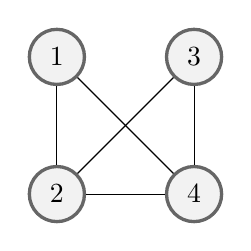
\begin{tikzpicture}[
    roundnode/.style={circle, draw=black!60, fill=gray!10, very thick, minimum size=7mm},
    ]

    \node[roundnode] (1) {1};
    \node[roundnode] (2) [below=of 1] {2};
    \node[roundnode] (3) [right=of 1] {3};
    \node[roundnode] (4) [below=of 3] {4};
    
    \draw[-] (3)--(4);
    \draw[-] (2)--(3);
    \draw[-] (4)--(2);
    \draw[-] (2)--(1);
    \draw[-] (1)--(4);
    \end{tikzpicture}

    \item $K_6$
    \item ~\\\includegraphics[scale = 0.4]{Homework/Images/treebipartitesecond.png}
    \item ~\\\includegraphics[scale = 0.4]{Homework/Images/treebipartite.png}
\end{qparts}
\begin{solution}
\begin{qparts}
    \item This graph is not a tree because trees do not contain cycles. $C_4$ is bipartite because there are no cycles with an odd number of nodes. We could have also showed an explicit 2-coloring to show that this graph is bipartite. 
    \item Since this graph contains cycles, it is not a tree. Additionally, this graph is not bipartite because it contains odd cycles, for example $(1,4,2).$ 
    \item Since $K_6$ contains cycles, it is not a tree. Additionally, it is not bipartite because there are cycles with an odd number of nodes. 
    \item Since this graph is connected and does not contain cycles, it is a tree. Additionally, since this graph contains no odd cycles, it is also bipartite.
    \item Since this graph is not connected (and it contains a cycle), it is not a tree. However, since this graph contains no odd cycles, this graph is bipartite. Additionally, we could have also shown an explicit 2-coloring to show that this graph is bipartite.
\end{qparts}

\textbf{Draft Grading Guidelines [20 points]}

\textbf{For each part:}
\begin{guidelines}
    \item +0.5 correct answer for tree
    \item +1 valid justification for tree
    \item +0.5 correct answer for bipartite
    \item +1 valid justification for bipartite
\end{guidelines}
\end{solution}

\subsection*{\probnum Road Rage [12 points]}
The graphs below shows some major roads in New Jersey. The graph on the left shows distances between cities on these roads, and the graph on the right shows the toll costs on each road.

\resizebox{\textwidth}{!}{
\includegraphics[]{Homework/Images/njroads.png} \includegraphics[]{Homework/Images/njtolls.png}
}

For each pair of cities below, (i) find the shortest path in distance, and (ii) find the least expensive route (shortest path in terms of cost). Be sure to list the total distance and total cost for each respective part.

\begin{qparts}
    \item Newark to Camden
    \item Trenton to Atlantic City
\end{qparts}

\begin{solution}
\begin{qparts}
    \item \begin{qsubparts}
        \item Shortest path: Newark $\rightarrow$ Woodbridge $\rightarrow$ Camden. Distance: 80.
        \item Least expensive route: Newark $\rightarrow$ Woodbridge $\rightarrow$ Camden. Cost: \$0.60.
    \end{qsubparts}

    \item \begin{qsubparts}
        \item Shortest path: Trenton $\rightarrow$ Camden $\rightarrow$ Atlantic City. Distance: 85.
        \item Least expensive route: Trenton $\rightarrow$ Asbury Park $\rightarrow$ Atlantic City. Cost: \$1.25.
    \end{qsubparts}
\end{qparts}

\smallskip
\textbf{Draft Grading Guidelines [12 points]}

\textbf{For each part:}
\begin{guidelines}
    \item +2 correct shortest path in terms of distance
    \item +1 correct total distance
    \item +2 correct least expensive path
    \item +1 correct total cost
\end{guidelines}
\end{solution}

\subsection*{\probnum Isomorphish? [12 points]}
Determine whether or not each of the following pairs of graphs are isomorphic. If yes, provide an isomorphism. If not, explain why and propose a change to one of the graphs that would make them isomorphic; you do not need to provide an isomorphism in this case.
\begin{qparts}
    \item ~\\\includegraphics[]{Homework/Images/isomorphisim_graph_1.png} \includegraphics[]{Homework/Images/isomorphisim_graph_2.png}
    \item ~\\\includegraphics[scale=.85]{Homework/Images/isomorphisim_graph_4.png} \includegraphics[scale=.85]{Homework/Images/isomorphisim_graph_3.png}
\end{qparts}
\begin{solution}
\begin{qparts}
    \item These graphs are isomorphic. $f\colon\{0,1,2,3,4\}\to \{a,b,c,d,e\}$ defined as follows is an isomorphism: $f(0)=a,$ $f(1)=b,$ $f(2)=e,$ $f(3)=d,$ $f(4)=c.$
    \item These graphs are not isomorphic. The left graph has 1 vertex with degree 5 while the right contains 2 vertices with degree 5. Adding an edge between vertices 6 and 3 to the left graph would make them isomorphic.
\end{qparts}

\smallskip
\textbf{Draft Grading Guidelines [12 points]}

\textbf{For each part:}
\begin{guidelines}
    \item +3 correct answer (are/are not isomorphic)
    \item +3 correct justification (provides isomorphism or valid change)
\end{guidelines}
\end{solution}

\newpage

\subsection*{\probnum Any tours available? [12 points]}
State whether each of the following contains, or is guaranteed to contain a Hamiltonian Cycle. Justify your response for each part. 
\begin{qparts}
    \item ~\\\includegraphics[width=3cm]{hamcycle_a.png} 
    \item ~\\\includegraphics[width=7.5cm]{hamcycle_b.png} 
    \item A simple, bipartite graph with 4 vertices that contains one cycle
    \item A 4-vertex graph where each vertex has even degree 
\end{qparts}

\begin{solution}
\begin{qparts}
    \item This graph contains a Hamiltonian Cycle. Ordering the vertices as follows will yield a Hamiltonian Cycle: $a,b,c,e,d,a.$
    \item This graph contains no Hamiltonian Cycle. One of the vertices $c$ or $f$ will always be visited twice or more when going through every vertex. 
    \item The only graph that follows this constraint is $C_4$, so this graph will always contain a Hamiltonian Cycle. 
    \item Not guaranteed to contain a Hamilton cycle. One counterexample is below:\\
    \includegraphics[width=3cm]{hamcycle_sol.png} 
\end{qparts}
\smallskip

\textbf{Draft Grading Guidelines [12 points]}

\textbf{For each part:}
\begin{guidelines}
    \item +1 correctly states whether there is a Hamiltonian cycle
    \item +2 correct justification 
\end{guidelines}
\end{solution}


\subsection*{\probnum Euler Visits the U.S. [12 points]}
Let $G=(V,E)$ be a graph of the continental U.S. where $V$ is the set of the first 48 states (excluding Alaska and Hawaii) and $E$ contains all pairs that share a border.  (Arizona and Colorado do not share a border, nor do Utah and New Mexico). A reference for the U.S. map has been provided below.

\begin{center}
    ~\\\includegraphics[width=15cm]
    {USMap1.png}
\end{center}

\begin{qparts}
    \item Does $G$ have an Euler path?  Prove or disprove.
    
    \item Is $G$ 3-colorable?  In other words, is there a function $f\colon V\rightarrow\{\text{red,blue,green}\}$ such that if $\{u,v\}\in E$ then $f(u)\neq f(v)$?

     \textbf{Hint:} Consider odd wheels $W_{2k + 1}$ 
    
\end{qparts}

\begin{solution}
\begin{qparts}
    \item{No, the graph has more than two vertices with odd degree, e.g., California, North Dakota, Maine.}
    
    \item No, $G$ is not 3-colorable. First we'll explain why odd wheels are not 3-colorable, and then we'll show that $G$ contains odd wheels. \\
    
    Why odd wheels are not 3-colorable: Attempting to 3-color $W_{2k+1}$, first color the center vertex. WLOG, we'll color it green. Since the center node shares an edge with every other node in the wheel, none of the other nodes can be green. Thus, the remaining $2k+1$ nodes (the ``outer nodes") must be colored with only \{red, blue\}. However, the remaining $2k+1$ nodes form an odd cycle, which is not 2-colorable. Therefore, odd wheels are not 3-colorable.\\
    
    $G$ contains odd wheels. For example, West Virginia and the surrounding states form a 5-wheel $W_5$.  Kentucky and the surrounding states form a 7-wheel.  Nevada and the surrounding states forms a 5-wheel. As a result, $G$ is not 3-colorable.
\end{qparts}
\textbf{Draft Grading Guidelines [12 points]}

\textbf{For each part:}
\begin{guidelines}
    \item +2 correct answer
    \item +4 correct justification
\end{guidelines}
\end{solution}


\subsection*{\probnum Ham and Cheese [15 points]}
A Hamiltonian cycle is a cycle that traverses through every vertex in a graph exactly once (starting and ending at the same vertex). How many Hamiltonian cycles are there in the complete graph $K_n$? Justify your answer.

\textbf{Note:} Two cycles are the same as long as the have the same vertices, and each vertex has the same left and right neighbors in the cycle. For instance the cycles $(a,b,c,a),$ $(b,c,a,b),$ and $(a,c,b,a)$ are all equivalent.

\begin{solution}
We have $n$ choices for picking the first vertex. From there we can visit any of the other $n-1$ vertices, so that gives us $n-1$ choices. The pattern follows until we're at the last vertex, where we have $1$ choice which is to return to our starting vertex. This yields
$$n\cdot (n-1)\cdot (n-2)\cdots 1 = n!$$
possible cycles.

However, we've overcounted: our current counting method treats $(a,b,c,a)$ and $(b,c,a,b)$ as two different cycles. For any particular cycle, there are $n$ possible starting vertices, so we need to divide by $n$ to account for this, yielding $(n-1)!$ possible cycles.

Unfortunately we're still overcounting! Even though we now count $(a,b,c,a)$ and $(b,c,a,b)$ as the same cycle, we still count $(a,b,c,a)$ and $(a,c,b,a)$ as distinct cycles even though they're really just the same cycle looping in the opposite direction. Note that for any cycle there are two possible ways we can traverse it, so $(n-1)!$ counts every cycle exactly twice. So our actual total number of cycles is
$$\frac{(n-1)!}2.$$

\textbf{Draft Grading Guidelines [15 points]}
\begin{guidelines}
    \item +4 starts with $n!$ cycles
    \item +4 divides by $n$ to account for the starting vertex
    \item +4 divides by 2 to account for orientation
    \item +3 correct final answer
\end{guidelines}
\end{solution}

\newpage


\subsection*{\probnum Captivating Counts [14 points]}
How many positive integers between $1000$ and $9999$ inclusive
\begin{qparts}
    \item have distinct digits?
    \item are divisible by 5 or 7?
    \item are divisible by 5 but not by 7?
\end{qparts}
Justify \textbf{and simplify} your answers. You may use a calculator to simplify.

\begin{solution}
\begin{qparts}
    \item 4536
    
    We can reason from left to right by considering each digit. There are 9 choices for the first (left-most) digit (since it cannot be a 0), then 9 choices for the second digit (since it cannot equal the first digit and we can now include 0), then, in a similar way, 8 choices for the third digit, and 7 choices for the right-most digit.  Therefore there are $9\cdot9\cdot8\cdot7 = 4536$ ways to specify such a number. In other words, there are $4536$ such numbers. Note that this coincidentally turns out to be almost exactly half of the numbers in the range.

    \item 2829
    
    There are $\lfloor \frac{999}{5}\rfloor$ multiples of 5 between 1 and 999, and similarly there are $\lfloor \frac{9999}{5}\rfloor$ between 1 and 9999. So there are $\lfloor \frac{9999}{5}\rfloor - \lfloor \frac{999}{5}\rfloor = 1999 - 199 = 1800$ multiples of 5 between 1000 and 9999, inclusive. Similarly there are $\lfloor \frac{9999}{7}\rfloor - \lfloor \frac{999}{7}\rfloor = 1428 - 142 = 1286$ multiples of 7 between 1000 and 9999, and $\lfloor \frac{9999}{5\cdot 7}\rfloor - \lfloor \frac{999}{5\cdot 7}\rfloor = 285-28 = 257$ multiples of both 5 and 7. So by the inclusion exclusion principle there are $1800 + 1286 - 257 = 2829$ multiples of 5 or 7 between 1000 and 9999.

    \item 1543
    
    We noted in the solution to part (c) that 1800 numbers are divisible by 5, and 257 of these are also divisible by 7. Therefore $1800 - 257 = 1543$ numbers in our range are divisible by 5 but not by 7.
\end{qparts}

\textbf{Draft Grading Guidelines [14 points]}

\textbf{Part a:}
\begin{guidelines}
    \item +1 counts without replacement
    \item +2 correct answer
    \item +1 some justification
\end{guidelines}
\textbf{Part b:}
\begin{guidelines}
    \item +2 correct counts of multiples of 5 and multiples of 7
    \item +1 correct count of multiples of $5\cdot 7$
    \item +2 correct final answer
    \item +1 some justification
\end{guidelines}
\textbf{Part c:}
\begin{guidelines}
    \item +1 attempts to use difference rule
    \item +2 correct final answer
    \item +1 some justification
\end{guidelines}
\end{solution}

\pagebreak
\section*{Grading of Groupwork \prevhwnum{}}
Using the solutions and Grading Guidelines, grade your Groupwork \prevhwnum{} Problems:
\begin{itemize}
    \item Use the table below to grade your past groupwork submission and calculate scores.
    \item While grading, mark up your past submission. Include this with the table when you submit your grading.
    \item Write whether your submission achieved each rubric item. If it didn't achieve one, say why not.
    \item For extra credit, write positive comment(s) about your work.
    \item You don't have to redo problems correctly, but it is recommended!
    \item See ``All About Groupwork" on Canvas for more detailed guidance, and what to do if you change groups.
\end{itemize}

\begin{center}
\resizebox{\textwidth}{!}{\begin{tabular}{| c | c | c | c | c | c | c | c | c | c | c | c | c |}
\hline
 & (i) & (ii) & (iii) & (iv) & (v) & (vi) & (vii) & (viii) & (ix) & (x) & (xi) & Total:\\
\hline
Problem 1 & & & & & & &\filcl &\filcl &\filcl & \filcl& \filcl& \hspace{1cm}/10\\
\hline 
Problem 2 & & & & & & &\filcl &\filcl &\filcl & \filcl& \filcl& \hspace{1cm}/8\\
\Xhline{1.25pt}
Total: &\filcl &\filcl &\filcl &\filcl &\filcl &\filcl &\filcl &\filcl & \filcl& \filcl& \filcl&\hspace{1cm}/18\\
\hline
\end{tabular}}
\end{center}

\pagebreak
\setcounter{probnumcount}{1}
\section*{Groupwork \hwnum{} Problems}

\subsection*{\probnum Commit Tea Party [15 points]} 
Two committees are having a meeting. If there are 12 people in each committee, how many different ways can they sit around a table given the following restrictions? Note that two orderings are considered equal if each person has the same two neighbors (without distinguishing their left and right neighbors).

\begin{qparts}
    \item There are no restrictions on seating.
    \item Two people in the same committee cannot be neighbors.
    \item Everybody must have exactly two neighbors from their committee.
    \item Everybody must have exactly one neighbor from their committee.
\end{qparts}

\begin{solution}
\begin{qparts}
    \item We can start by ordering the people in a line and then dividing to get rid of the overcounting caused by the symmetry of the table. Our initial count is $24!$ since that is the number of ways to arrange 24 people in a line.
    
    We then need to divide by 24. Imagine taking the line we counted and wrapping it around a table. Now we could rotate this table 24 times and it'd still be the same table. But counting the number of lines of people counts each rotation as a different line. So we overcounted by a factor of 24.

    Additionally, we need to divide by 2. Now imagine drawing a line between two people who are directly across from each other at the table. If we ``flip" everyone else across this line, we end up with the same table (everyone keeps the same two neighbors). But our numerator counted this arraignment as a different line. So we also have to divide by 2 to fix this.

    So our final answer is
    $$\frac{24!}{2\cdot 24}.$$
    
    \item For this to be the case the members of each committee must alternate in placement around the table.
    
    \textbf{Solution 1:} $\frac{2\cdot 12!\cdot 12!}{2\cdot 24}$ or $\frac{24\cdot 11!\cdot 12!}{2\cdot 24}$
    
    Like part (a), we can start by counting the ways to order people in a line and then divide that to account for overcounting.
    
    One way to get an initial count is to note that if the line starts with someone from committee A, then we have 12 choices for the first spot, 12 for the second (this person has to be committee B), 11 for third (now person needs to be on committee A again), and so on. This gives us $12! \cdot 12!$. Similarly we get $12!\cdot 12!$ options if the line starts with someone from committee B. So that gives us a count of $2\cdot 12!\cdot 12!$

    Another way to get our initial count is to note that the first person in the line can be anyone (24 options), then there are 12 options for the second spot (12 people on the other committee), then 11 options for the third spot (11 people on the same committee as the first person), etc. This product give us $24\cdot 12\cdot 11\cdot 11\cdot 10\cdots 1 = 24\cdot 12!\cdot 11!$

    We then need to divide by $2\cdot 24$ by the same logic as (a), yielding a final count of
    $$\frac{2\cdot 12!\cdot 12!}{2\cdot 24}.$$
    
    \textbf{Solution 2:} $\frac{11! \cdot 12!}{2}$
    
    Imagine the same person from the group always sits down first, let's call them Frank. Frank can sit anywhere in the table. After Frank sits down, there are only 12 options for the person sitting to Frank's left. Then the spot after that has 11 options (has to be from Frank's committee). The spot after that also has 11 options (has to not be from Frank's committee). Working around the table gives us $12!\cdot 11!$ 
    
    However we still have the issue of overcounting for symmetry, so we need to divide by 2 to get $\frac{11! \cdot 12!}{2}.$ On the other hand, we don't have the issue of overcounting for rotations because we didn't distinguish between the different options for Frank's seat. If instead we had said that Frank has 24 options at the start, then we'd have to divide to get $\frac{24\cdot 11!\cdot 12!}{2\cdot 24}.$
    
    \item 0. This is impossible. Even if we separate the committees as much as possible at least two people need to sit next to someone who's not on their committee 
    
    \item \textbf{Incorrect Solution:}
    
    Let this be a cautionary tale that counting problems are sometimes very nuanced and tricky! We originally published that we can get this answer by subtracting our answers of parts (b) and (c) from part (a). The thinking was that (no restrictions) - (0 neighbors from same committee) - (2 neighbors from same committee) would equal 1 neighbor from same committee. But this doesn't account for cases where some people have 1 neighbor from their committee and some people have two. Example: the case where half of the table is one committee and half the table is the other committee was incorrectly counted in our original answer.
    
    \textbf{Correct Solution:}
    
    It seems easiest to count this directly, similar to part (b). So first count the ways to order people in a line then divide by the overcounting. 
    
    \emph{Solution 1:} If we use the same denominator as above, $2\cdot 24$, then the numerator needs to count all possible lines of people where each person has exactly one neighbor. So there are two cases for the numerator, our initial count:
    \begin{stmts}
        \item The first two people in the line belong to the same committee For example with committees A and B the line looks like AABBAA... or BBAABB....

        There are 24 options for the first person and 11 options for the second. Then the third person has to be from the other committee, so there are 12 options. The 4th person has to be from the same committee as the third, so 11 options. The 5th person has to be from the same committee as the first person, so 10 options. And so on. This gives us $24\cdot 11! \cdot 12!$

        \item The first two people in the line belong to different committees. For example with committees A and B the line looks like ABBAABB... or BAABAA....
        
        There are 24 options for the first person and 12 options for the second. The third person has 11 options because they have to be from the same committee as the second person. The 4th person has 11 options because they have to be from the same committee as person 1. This gives us $24\cdot 12! \cdot 11!$
    \end{stmts}
    This yields a final answer of
    $$\frac{2\cdot 24\cdot 12! \cdot 11!}{2\cdot 24}.$$
    
    \emph{Solution 2:} Instead of counting all possible lines of people in the numerator, we can just count the number of ways to have the line look like AABBAABB... (of which there are $12!\cdot 12!$ ways). Now this numerator only overcounts each string by 6 for the different rotations around the circle, and we still have overcounting by 2 for symmetry. 
    
    So our final answer is
    $$\frac{12!\cdot 12!}{2\cdot 6}.$$
    
    Note: to more rigorously prove this we should use induction to prove that AABBAA... will generate all such seating arraignments, but that is not something we expect you to do.
\end{qparts}

\textbf{Draft Grading Guidelines [15 points]} 

\textbf{Part a:}
\begin{gwguidelines}
    \item +2 correct numerator with justification
    \item +2 correct denominator with justification
\end{gwguidelines}
\textbf{Part b:}
\begin{gwguidelines}[resume]
    \item +2 correct numerator with justification
    \item +2 correct denominator with justification
\end{gwguidelines}
\textbf{Part c:}
\begin{gwguidelines}[resume]
    \item +3 correctly explains that this is impossible
\end{gwguidelines}
\textbf{Part d:}
\begin{gwguidelines}[resume]
    \item +2 correct numerator with justification
    \item +2 correct denominator with justification
\end{gwguidelines}
\end{solution}


\subsection*{\probnum Hiking Extravaganza [15 points]}
Prove that every complete $n$-node weighted graph (with all possible edges) with $n \ge 1$ and all distinct edge weights has a (possibly non-simple) path of $n-1$ edges along which the edge weights are strictly increasing.

\textbf{Hint:} Start by placing a hiker on each node. Try to show that the sum of the number of edges traversed by each hiker is $n(n-1)$, each along increasing-weight paths.

\begin{solution} 
Place a hiker at each node of $G$. Consider the edges of $G$ in order of increasing weight. When each edge $\{u, v\}$ is considered, have the hiker currently at $u$ walk across the edge to $v$, and the hiker currently at $v$ walk across the edge to $u$ (so they switch places). At the end of this process, each edge will have traversed by exactly 2 hikers (one in each direction). 

Because our process visits the edges in order of increasing weight, \textbf{the path walked by each hiker is guaranteed to be an increasing-weight path.}

Next we want to show that at least one hiker's path contained (at least) $n-1$ edges. To do this, we'll first consider average number of edges in a hiker's path. 
\begin{itemize}
    \item The sum of the edges traversed by all hikers is twice the number of edges in the graph, since each edge was traversed by 2 hikers (one in each direction).
    \item The total number of edges can be found in a variety of ways, including via the Handshake Theorem, which we do here. The Handshake theorem tells us that the sum of the degrees in a graph is twice the number of edges. For a complete graph on $n$ nodes, each node has degree $n-1$. The sum of degrees is $n(n-1)$, so the total number of edges is $\frac{n(n-1)}{2}.$  
    \item So the sum of the edges traversed by all hikers is $2\cdot \frac{n(n-1)}{2} = n(n-1).$
    \item The average number of edges in a hiker's path is then $\frac{n(n-1)}{n}=n-1.$
\end{itemize} 

Since the average edges-in-path is $n-1$, then at least one hiker must have walked a path with $\ge n-1$ edges. (Because that's how averages work.) 

This process is demonstrated below for $C_{3}$ and $C_{4}$:

\includegraphics[width=0.6\textwidth]{hiking.png}

\textbf{Grading Guidelines [15 points]}
\begin{gwguidelines}
    \item +4 goes over edges in increasing order
    \item +3 swaps hikers along each edge
    \item +3 notes that in total the hikers takes $n(n-1)$ steps
    \item +5 deduces that there must be one hiker with $ \geq n - 1$ steps
\end{gwguidelines}
\end{solution}

\end{document}
